\documentclass[a4paper,12pt]{article}
\usepackage[utf8]{inputenc}
\usepackage{amsmath}
\usepackage{amssymb}
\usepackage{hyperref}
\usepackage{geometry}
\usepackage{graphicx}
\geometry{margin=1in}

\title{Homework 4:\\A New Golden Age for Computer Architecture}
\author{Pupipat Singkhorn}
\date{\today}

\begin{document}

\maketitle

\section*{Introduction}

We live in a world that is constantly changing. As you graduate from this course, you should keep up with current trends and emerging techniques. This assignment serves as a practice for your lifelong learning journey. You will read a review article that talks about the past, the present, and the future of computer architecture. Even though the past might seem boring and irrelevant at first, you will notice that many of the techniques in the past keep reappearing in new forms. This is true in many fields of study.
You will find many concepts that we learned in the course, and it should serve as a good review.
This exercise will have you read and answer questions based on a recent article by computer architecture experts, John L. Hennessy and David A. Patterson.
You can access the article by going to the materials section in MCV.
Lastly, important concepts from this article will also appear in the final exam.

\section*{Questions}

\begin{enumerate}
    \item According to the CPU time formula, why is RISC better than CISC?

    \textbf{Answer:}
    \[
    \text{CPU Time} = \text{Instruction Count} \times \text{Cycles Per Instruction (CPI)} \times \text{Cycle Time}
    \]
    \begin{enumerate}
        \item Lower CPI: simpler instructions, but at the cost of the number of instructions.
        \item Faster clock: shorter cycle time.
    \end{enumerate}

    \item Why did the `Itanic' ISA become unused?

    \textbf{Answer:}
    It struggled to achieve high performance for integer programs that had less predictable cache misses or less-predictable branches.
    It also faced challenges with x86 compatibility and market adoption.

    \item What type of parallel architecture according to Flynn's taxonomy is Itanic?

    \textbf{Answer:}
    Multiple Instruction Multiple Data (MIMD)

    \newpage

    \item Explain `Dennard scaling' in your own words.

    \textbf{Answer:}
    \[
    \text{Power density} = \frac{\text{Power}\ (\downarrow)}{\text{Area}\ (\downarrow)} = \text{Constant}
    \]
    Transistors get smaller(area decrease), their power density(power/area) stays constant.

    \item Why is it not practical to keep increasing the number of pipeline stages and thus increasing the ILP?

    \textbf{Answer:}
    \begin{enumerate}
        \item \textbf{Branch Misprediction Inefficiency}: Increasing ILP amplifies the impact of branch mispredictions, leading to wasted computational work and energy.

        \item \textbf{Accuracy Challenge}: Achieving high prediction accuracy is particularly difficult for general-purpose programs with unpredictable branching patterns.

        \item \textbf{Limited Practical Gains}: Frequent mispredictions reduce the performance and energy efficiency benefits of increased ILP, making it less practical for most workloads.
    \end{enumerate}

    \item According to Figure 5, when 8\% of the time is serial, what is the percentage of energy wasted by a 45-processor configuration?

    \textbf{Answer:}

    \begin{figure}[h]
        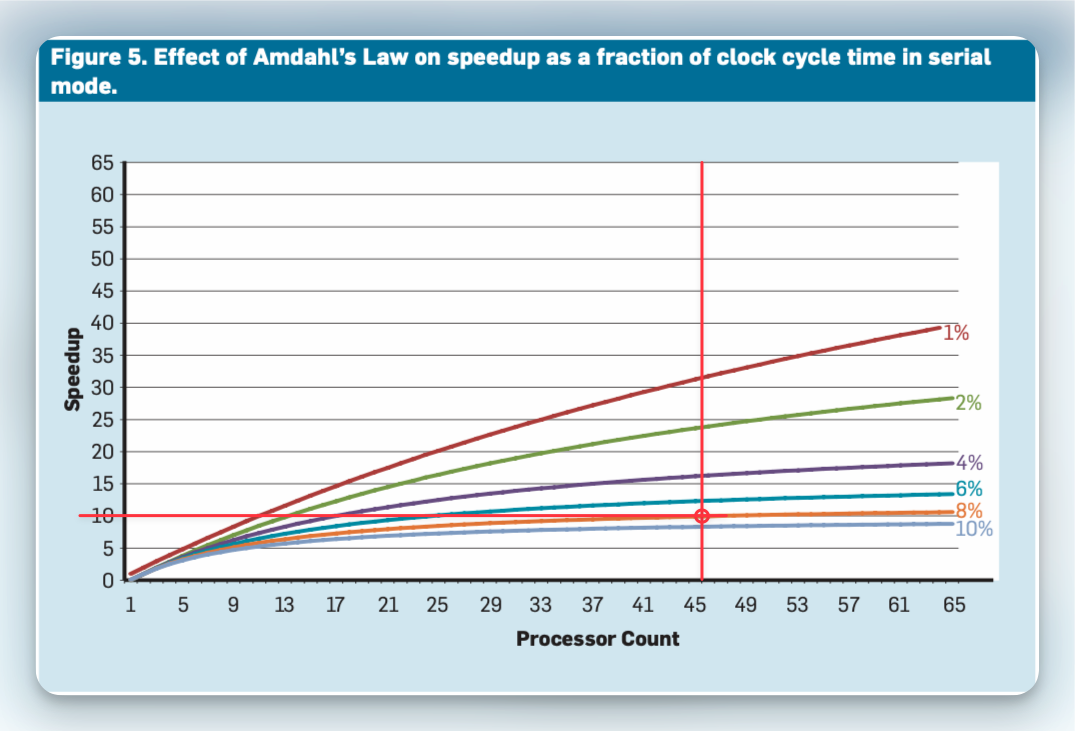
\includegraphics[width=10cm]{fig5.png}
        \centering
    \end{figure}

    \[
    \therefore \text{Energy Wasted} = 1 - \frac{10}{45} = 0.7778 = 77.78\%
    \]

    \item Why can VLIW be a good fit for DSA?

    \textbf{Answer:}
    VLIW (Very Long Instruction Word) suits DSAs (Domain-Specific Architectures) as it exploits predictable parallelism, simplifies hardware by relying on static scheduling, and achieves energy efficiency, making it ideal for specialized, repetitive workloads.

    \newpage

    \item What is your impression regarding Figure 7? Does it change your view of how to program? What are the things that you should be aware of in order to write more efficient software?

    \textbf{Answer:}

    \textbf{Impression of figure 7.}\\
    It shows a dramatic and significant performance improvement, with approximately a 10x speedup from Python to C and up to a 60,000x boost using SIMD optimization.

    \textbf{Does it change my view of how to program?}\\
    Yes, it reinforces the importance of understanding the underlying hardware and choosing the right tools and techniques for computationally intensive tasks.

    \textbf{Things to be aware of to write more efficient software.}
    \begin{enumerate}
        \item Choose the right language
        \item Leverage parallelism
        \item Optimize memory usage
        \item Hardware-specific features
    \end{enumerate}

    \item Explain what systolic arrays are. How are systolic arrays different from typical SIMD architectures? When were they first created? You should read other sources to get a better understanding of them. Write down the sources you used.

    \textbf{Answer:}

    \textbf{Explain what systolic arrays are.}\\
    Systolic arrays are specialized hardware architectures designed to perform parallel computations efficiently. They consist of a network of processing elements (PEs) connected in a regular grid, where data flows synchronously between PEs in a rhythmic, "systolic" manner (similar to a heartbeat). Each PE performs a specific operation and passes the result to its neighbor.
    \begin{figure}[h]
        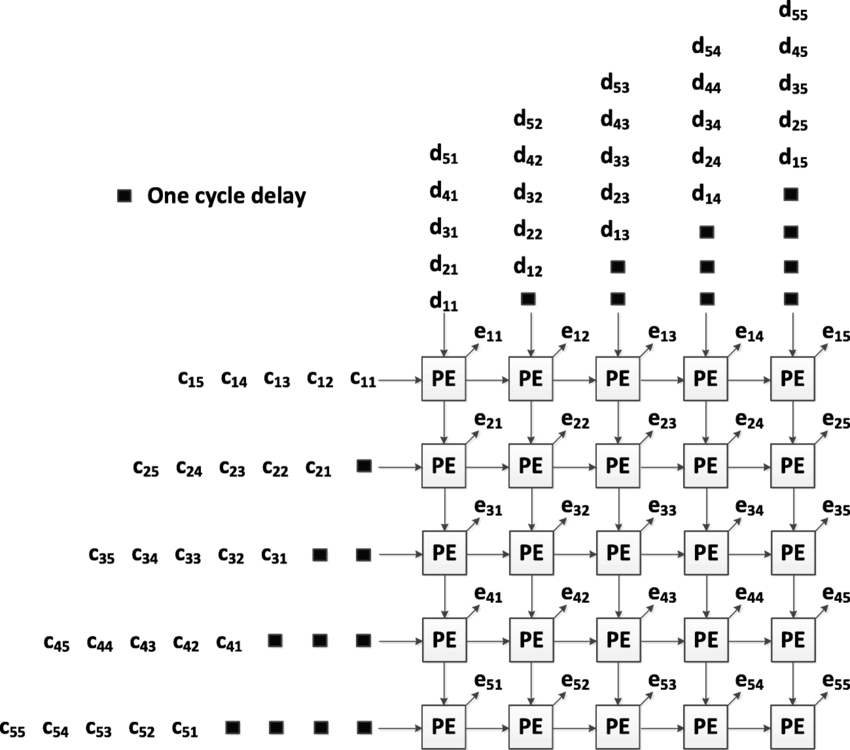
\includegraphics[width=5cm]{55-Systolic-array-architecture.png}
        \centering
    \end{figure}

    \textbf{How are systolic arrays different from typical SIMD architectures?}\\
    Systolic arrays move data rhythmically through synchronized processing elements (PEs), ideal for structured tasks like matrix operations, with direct PE-to-PE communication. SIMD architectures broadcast a single instruction to all units, excelling in data-parallel tasks like image processing, using memory or buses for communication. Each is suited to different computational needs.

    \newpage

    \textbf{When were they first created? }\\
    Systolic arrays were first conceptualized by H.T. Kung and Charles E. Leiserson in the late 1970s. The concept was formally introduced in their 1979 paper, "Algorithms for VLSI Processor Arrays."

    (Sources: In the references section.)

    \item Explain the similarities and differences between Agile software development and Agile hardware development.

    \textbf{Answer:}
    \begin{enumerate}
        \item \textbf{Similarities}: Both Agile software and hardware development focus on iterative cycles, collaboration, flexibility, prototyping, and delivering incremental improvements.

        \item \textbf{Differences}: Software iterations are faster and cheaper, with virtual testing and easy post-deployment updates. Hardware involves slower cycles, higher costs, physical prototyping, and limited flexibility after production.

        \item \textbf{Conclusion}: Agile principles apply to both, but hardware faces more constraints due to its physical nature.
    \end{enumerate}

\end{enumerate}

\subsection*{References}

\begin{enumerate}
    \sloppy
    \item \url{https://cs.stanford.edu/people/eroberts/courses/soco/projects/risc/risccisc/}
    \item \url{https://www.sciencedirect.com/topics/computer-science/systolic-arrays}
    \item \url{https://en.wikipedia.org/wiki/Systolic_array}
    \item \url{https://www.researchgate.net/figure/55-Systolic-array-architecture_fig3_343586463}
    \item \url{https://en.wikipedia.org/wiki/Flynn%27s_taxonomy}
    \item \url{https://en.wikipedia.org/wiki/Dennard_scaling}
    \item \url{https://en.wikipedia.org/wiki/Itanium}
    \item \url{https://chatgpt.com/}
\end{enumerate}

\end{document}